\documentclass[../piano-di-progetto.tex]{subfiles}
\begin{document}
\subsection{Progettazione della technology baseline}
Il periodo di progettazione della technology baseline inizia il 2020-04-21, dopo la revisione dei requisiti, e termina il giorno 2020-04-26 con l'inizio del primo incremento. 

\subsubsection{Ruoli}
Durante questa macro, viene richiesta la presenza dei seguenti ruoli:
\begin{itemize}
    \item Responsabile;
    \item Amministratore;
    \item Analista;
    \item Progettista;
    \item Verificatore.
\end{itemize}

\subsubsection{Attività}
Questa macro è composta da un unico periodo:
\\
\\
\textbf{Periodo unico (2020-04-21 - 2020-04-26)}:
        \begin{itemize}
            \item Revisione ed eventuale aggiornamento dei seguenti documenti:
            \begin{itemize}
                \item \textsc{Norme di progetto v1.0.0-old};
                \item \textsc{Analisi dei requisiti v1.0.0-old};
                \item \textsc{Piano di progetto v1.0.0-old};
                \item \textsc{Piano di qualifica v1.0.0-old}.
            \end{itemize}

            \item \textbf{Ricerca degli strumenti}: studio autonomo degli strumenti richiesti per lo sviluppo del progetto; 
            \item \textbf{Progettazione}: progettazione dell'architettura di sistema;
            \item \textbf{Verifica}.
        \end{itemize}
    
    


\newpage
\begin{landscape}
    \begin{figure}[H]
        \centering
        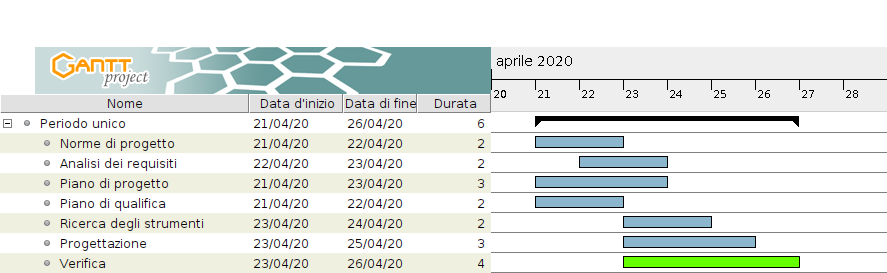
\includegraphics[width=24cm]{img/progettazione.png}
        \caption{Diagramma attività nel periodo di progettazione della technology baseline}
      \end{figure}
\end{landscape}

    
\newpage
\subsection{Realizzazione del Proof of Concept}

Durante questo macro-periodo verranno implementate alcune tra le funzionalità più importanti richieste dal proponente. Verranno svolti quattro incrementi che produrranno un Proof of Concept. Viene richiesta la presenza di tutti i ruoli per ognuno dei quattro incrementi.

\subsubsection{I incremento} 

 Vengono stabiliti i seguenti obiettivi per il primo incremento:
 \begin{itemize}
     \item Installazione e configurazione di Grafana;
     \item Installazione e configurazione dell'ambiente di sviluppo \glossario{Node} e del framework \glossario{Electron}.
 \end{itemize}
 
\paragraph{Attività}
Le attività verranno svolte in un unico periodo:
\\
\\
\textbf{Periodo unico (2020-04-27 - 2020-04-29):}
\begin{itemize}
    \item Progettazione;
    \item Codifica: implementazione delle funzionalità progettate;
    \item Verifica: controllo delle funzionalità implementate.
\end{itemize}

\subsubsection{II incremento}
 
 
 Vengono stabiliti i seguenti obiettivi per il secondo incremento:
 \begin{itemize}
     \item Creazione del \glossario{front-end} del programma di addestramento;
     \item Integrazione del framework Electron per l'avvio dell'applicazione.
 \end{itemize}
\paragraph{Attività}
Le attività verranno svolte in un unico periodo:
\\
\\
\textbf{Periodo unico (2020-04-30 - 2020-05-02):}
\begin{itemize}
    \item Progettazione;
    \item Codifica: implementazione delle funzionalità progettate;
    \item Verifica: controllo delle funzionalità implementate.
\end{itemize}


\subsubsection{III incremento}

 Vengono stabiliti i seguenti obiettivi per il terzo incremento:
 \begin{itemize}
     \item Implementazione dell'algoritmo di RL per la generazione dei \glossario{predittori} nel programma di addestramento;
     
     \item Implementazione della logica applicativa per l'input dei dati nel programma di addestramento e l'output dei predittori;
 \end{itemize}
 
\paragraph{Attività}
Le attività verranno svolte in un unico periodo:
\\
\\
\textbf{Periodo unico (2020-05-03 - 2020-05-06):}
\begin{itemize}
    \item Progettazione;
    \item Codifica: implementazione delle funzionalità progettate;
    \item Verifica: controllo delle funzionalità implementate.
\end{itemize}


\subsubsection{IV incremento}

 Vengono stabiliti i seguenti obiettivi per il quarto incremento:
 \begin{itemize}
     \item Implementazione del front-end del plug-in Grafana per la visualizzazione dei dati in grafici e indici.
 \end{itemize}
\paragraph{Attività}
Le attività verranno svolte in un unico periodo:
\\
\\
\textbf{Periodo unico (2020-05-07 - 2020-05-10):}
\begin{itemize}
    \item Progettazione;
    \item Codifica: implementazione delle funzionalità progettate;
    \item Lettera di presentazione;
    \item Consuntivo di periodo;
    \item Realizzazione di un video dimostrativo;
    \item Verifica: controllo delle funzionalità implementate e dei documenti.
\end{itemize}



\newpage
\begin{landscape}
    \begin{figure}[H]
        \centering
        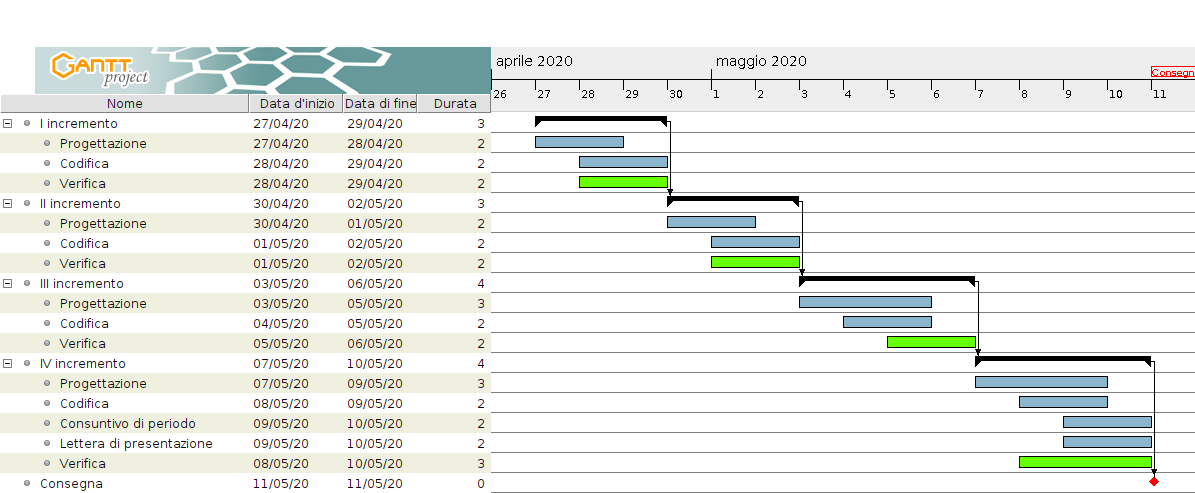
\includegraphics[width=24cm]{img/poc.png}
        \caption{Diagramma attività nel periodo di realizzazione della Proof of Concept}
      \end{figure}
\end{landscape}

\end{document}
